%%
%% Dokumentenart
%%
\NeedsTeXFormat{LaTeX2e}
\documentclass[
    a4paper,
    10pt,
    bibliography=totoc,
    twoside,
    openright,
    numbers=noenddot,
    headings=normal,
    DIV=9,
    parskip
    %,draft
]{scrbook}


%%
%% Unterstützung für deutsche Sprache, Umlaute etc.
%%
\usepackage[utf8]{inputenc}
\usepackage[T1]{fontenc}
\usepackage[ngerman]{babel}
\usepackage[babel,german=quotes]{csquotes}


%%
%% Diverse Pakete
%%
\usepackage{scrhack}
\usepackage{graphicx}
\usepackage{verbatim}
\usepackage{tabularx}
\usepackage{subfigure}
\usepackage{url}
\usepackage{color}
\usepackage{amssymb}
\usepackage{amsmath}
\usepackage{amsthm}
\usepackage{setspace}
\usepackage{listings}
\usepackage{colortbl}
%\usepackage{showframe} % Seitenspiegel anzeigen
\usepackage{microtype}
\usepackage{hyperref} % muss letztes Paket in der Liste sein


%%
%% hier Namen etc. einsetzen
%%
\newcommand{\fullname}{Merve Bayirli, Julian Heyne, Payam Ebadi}
\newcommand{\email}{merve.bayirli@uni-ulm.de, julian.heyna@uni-ulm.de, ...}
\newcommand{\titel}{Playing Minesweeper with
Reinforcement Learning in Neural Networks}
\newcommand{\jahr}{2017}
\newcommand{\matnr}{790102, 654, 654}
\newcommand{\gutachterA}{Dr.\ Fridhelm Schwenker}
%\newcommand{\gutachterB}{Prof.\ Dr.\ Un Leserlich}
%\newcommand{\betreuer}{Betreuername}
\newcommand{\fakultaet}{Ingenieurwissenschaften\\und Informatik}
%\newcommand{\fakultaet}{Mathematik und\\Wirtschaftswissenschaften}
%\newcommand{\fakultaet}{Naturwissenschaften}
%\newcommand{\fakultaet}{Medizin}
\newcommand{\institut}{Institut für Neuroinformatik}
\newcommand{\arbeit}{Projektarbeit}
%\newcommand{\arbeit}{Bachelorarbeit}


%%
%% Setzt Autor und Titel in den Metadaten des erzeugten Dokumentes
%%
\pdfinfo{
    /Author (\fullname)
    /Title (\titel)
    /Producer (pdfeTex 3.14159-1.30.6-2.2)
    /Keywords ()
}
\hypersetup{
    pdftitle=\titel,
    pdfauthor=\fullname,
    pdfsubject={\arbeit},
    pdfproducer={pdfeTex 3.14159-1.30.6-2.2},
    colorlinks=false,
    pdfborder=0 0 0
}


%%
%% Tiefe, bis zu der Überschriften in das Inhaltsverzeichnis kommen
%%
\setcounter{tocdepth}{3}


%%
%% Verhindert überhängende Absatzteile
%%
\clubpenalty10000
\widowpenalty10000
\displaywidowpenalty=10000


%%
%% Einstellungen für Codelistings
%%
\lstset{
    language=Java,
    showstringspaces=false,
    frame=single,
    numbers=left,
    basicstyle=\ttfamily,
    numberstyle=\tiny
}


%%
%% Formatierung des Literaturverzeichnisses
%%
\bibliographystyle{plaindin} % Nummern und alphabetisch sortiert
%\bibliographystyle{alphadin} % Buchstaben und sortiert
%\bibliographystyle{abbrvdin} % Nummern und abgekürzte Namen
%\bibliographystyle{unsrtdin} % Nummern und unsortiert


%%
%% Eigene Makros
%%
\newcommand{\FIXME}[1]{\colorbox{yellow}{\bf FIXME: #1}}


%%
%% Eigene Farben
%%
\definecolor{Gray}{rgb}{0.80784, 0.86667, 0.90196} %dunkelblau
\definecolor{Lightgray}{rgb}{0.9176, 0.95, 0.95686} %hellblau
\definecolor{Akzent}{rgb}{0.6627, 0.63529, 0.55294} %akzentfarbe


%%
%% Liniendicke in Tabellen etc.
%%
\setlength{\arrayrulewidth}{0.1pt}


%%
%% Schriftarten
%%
\renewcommand{\sfdefault}{phv}
\renewcommand{\rmdefault}{phv}
\renewcommand{\ttdefault}{pcr}
\KOMAoptions{DIV=last}


%%
%% Seitenlayout
%%
\pagestyle{headings}


%%
%% Trennungsregeln
%%
\hyphenation{Sil-ben-trenn-ung}


%%
%% Schönere Bullets bei Aufzählungen
%%
\renewcommand{\labelitemi}{$\bullet$}
\renewcommand{\labelitemii}{$\circ$}
\renewcommand{\labelitemiii}{$\cdot$}


%%
%% Beginn des eigentlichen Dokumentes
%%
\begin{document}


%%
%% Vorspann
%%
\frontmatter


%%
%% Titelseite
%%
\thispagestyle{empty}
\begin{addmargin*}[4mm]{-32mm}
    % Logo und Wortmarke
    
\includegraphics[height=1.8cm]{images/unilogo_bild}
    \hfill
    
\includegraphics[height=1.8cm]{images/unilogo_wort}
    \vspace*{2.1em}

    % Briefkopf
    \footnotesize
    \textbf{Universität Ulm} \textbar ~89069 Ulm \textbar ~Germany
    \hfill
    \parbox[t]{42mm}{\bfseries Fakultät für\\\fakultaet\\\mdseries\institut}
    \vspace*{2cm}

    % Titel
    \parbox{140mm}{\bfseries \raggedright \huge \titel}

    % Untertitel
    {\arbeit{} an der Universität Ulm}
    \vspace*{4em}

    % Prüfer etc.
    \textbf{Vorgelegt von:}\\\fullname\\\email\\[2em]
    \textbf{Gutachter:}\\\gutachterA\\[2em]
%    \textbf{Betreuer:}\\\betreuer\\[1.5em]
    \jahr
\end{addmargin*}


%%
%% Impressum
%%
\clearpage
\thispagestyle{empty}
{
    % vollständiger Titel
    \small \flushleft \enquote{\titel}\\
    Fassung vom \today
    \vfill

    % Danksagung
    %\textsc{Danksagungen:}
    %\FIXME{Danksagungen}
    \vspace{1cm}

    % Anerkennung
    Bei der Erstellung dieser \arbeit{} wurde ausschließlich freie Software eingesetzt: \\
    \begin{figure}[ht]
        \centering
        \subfigure{
\includegraphics[height=1cm]{images/sw/ubuntu}}
        \hspace{0.5cm}
        \subfigure{
\includegraphics[height=1cm]{images/sw/texmaker}}
        \hspace{0.5cm}
        \subfigure{
\includegraphics[height=1cm]{images/sw/inkscape}}
        \hspace{0.5cm}
        \subfigure{
\includegraphics[height=1cm]{images/sw/subversion}}
        \hspace{0.5cm}
        \subfigure{
\includegraphics[height=1cm]{images/sw/jabref}}
        \hspace{0.5cm}
        \subfigure{
\includegraphics[height=1cm]{images/sw/firefox}}
        \hspace{0.5cm}
        \subfigure{
\includegraphics[height=1cm]{images/sw/evince}}
    \end{figure}
    \vspace{1cm}

    % Urheberrechtshinweis
    \copyright{} \jahr{} \fullname{}\\[0.5em]
    % Falls keine Lizenz gewünscht wird bitte den folgenden Text entfernen.
    % Die Lizenz erlaubt es zu nichtkommerziellen Zwecken die Arbeit zu
    % vervielfältigen und Kopien zu machen. Dabei muss aber immer der Autor
    % angegeben werden. Eine kommerzielle Verwertung ist für den Autor
    % weiter möglich.
    Dieses Werk ist unter der Creative Commons Attribution-NonCommercial-ShareAlike 3.0 Germany License lizensiert: \url{http://creativecommons.org/licenses/by-nc-sa/3.0/de/}\\
    Satz: PDF-\LaTeXe{}\\
%    Druck: \FIXME{Druck}
}


%%
%% Inhaltsverzeichnis
%%
\setstretch{1.4}
\tableofcontents


%%
%% Hauptteil
%%
\mainmatter
\chapter{Introduction}

\section{Motivation}
Reinforcement Learning is an interesting field of machine learning. An agent learns which
actions to take in an environment given certain rewards. However, the naive algorithms
struggle with high--dimensional sensory input. One way to bypass this problem is the
usage of handcrafted features. These systems are unfortunately not easily applicable
to other problems and highly dependent on the quality of the feature representation. Deep
learning makes it possible to extract higher levels of abstractions from raw sensory input.
These techniques are for example used by Google Deepmind to play seven, and later 49 Atari games with a deep Q--network~\cite{mnih2013playing, mnih2015human}.
Minesweeper is a game almost everyone, who used Microsoft Windows, knows. 
This makes it an interesting subject for a project applying reinforcement learning. Playing
it with a deep reinforcement learning approach enables to learn more in the fields of reinforcement as well as deep learning.

\begin{figure}
	\centering
	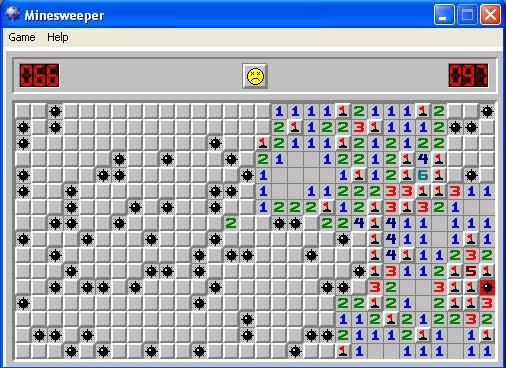
\includegraphics[scale=0.8]{images/img_26041_minesweeper_large.jpg}
	\caption{Minesweeper game played on Windows.}
	\label{fig:minesweeper}
\end{figure}

\section{Minesweeper}
Minesweeper is a video game which was introduced in the $1960$s. 
While Minesweeper looks like an easy game to play, simply checking a board state for consistency is a NP--complete problem.
Deciding which action to take requires logical, arithmetic and as not each decision can be decided by pure logic also probabilistic reasoning.
Human performance is far from optimal~\cite{castillo2003learning}.

The game is represented by equally looking squares that are arranged on a grid. 
Some of the squares contain mines which were randomly assigned at the start of the game. 
At the beginning of every game the grid size as well as the number of mines on the grid is known.
The player can select one of the squares. 
If a square that contains a mine is chosen the game is lost.
Else the square will show a digit from $0$ to $8$.
This digit represents the number of mines that surround the chosen field.
In other words if no field with a mine is adjacent to the chosen one, the chosen one has the digit $0$. 
If all the adjacent squares contain mines the digit will be $8$.
A game is won if all squares without mines are open.
In the original game the player can not only choose to open a square he can also 'flag' or 'unflag' a field.
This means, that if the player is sure that a field contains a mine he can flag it to mark that that field contains a mine.
The flagging is only needed for human players as they are the only way to track mines throughout the game.
The agent does not need a specific way to mark mines with flags and removing this option halves the actions the agent can take.
Additionally we tested the use of flagging in some early games and noticed heavy deadlocking in games.
Flagging a field did not change that much in a state and thus the most probable action after flagging was repeating the same action.
Thus we chose to not have flags as possible actions.

\section{Previous Work}
While Minesweeper is a well--known game, it has not seen much research especially in reinforcement learning.
One paper, that we found is not based on reinforcement learning but instead it is based on multirelational learning~\cite{castillo2003learning}.
They use a general purpose learning system (MIO) and use it to learn from examples in clausal logic.
They were able to beat the performance of human players on an $8\times8$ field with $10$ mines.
% hier weitere Kapitel einbinden
\chapter{Deep-Reinforcement Learning}
Our first attempt to solve the problem of a neural network playing minesweeper is with deep--reinforcement learning.
Techniques able to learn Atari games~\cite{mnih2013playing} with a high input complexity should be able to learn and play `simpler' games like Minesweeper.
First we introduce the concept of Reinforcement learning with the addition of Deep Reinforcement Learning.
Afterwards we present our approach, followed by our results and the problems we encountered.

\section{Background}
Reinforcement learning is used to learn an optimal policy for an agent in an environment by exploring the environment and getting rewards based on its performance.
The environment $\mathcal{E}$ can be regarded as a sequence of actions, states and rewards.
At every time--step the agent selects a legal action $a_t$ from a set of legal game actions. 
The goal of the agent is to maximize the future reward.
We use as the future reward, the standard future discounted reward
\begin{equation}
R_t := \sum_{t'=t}^T \gamma^{t'-t}r_{t'},
\end{equation}
where $\gamma$ is a discount factor per time--step, $r_t$ represents the change in the game score and $T$ is the time--step at which the game is terminated.
The optimal action--value function $Q^*\left(s,a\right)$ is defined as the maximum expected return that will be returned by following any strategy:
\begin{equation}
Q^*\left(s,a\right):= \max_\pi \mathbb{E} \left[ R_t|s_t=s\text{, }a_t=a\text{, } \pi\right]
\end{equation}
where $s$ is some sequence and $\pi$ is a policy mapping sequences to actions.
%TODO belmann intuition erklären??
The optimal action--value function is gained with the Bellman equation by maximizing the expected value of $r+\gamma Q^*\left(s',a'\right),$
\begin{equation}
Q^*\left(s,q\right)= \mathbb{E}_{s' \sim \mathcal{E}} \left[ r + \gamma \max_{a'} Q^*\left(s',a'\right)| s,a \right],
\end{equation}
where $Q^*\left(s,a\right)$ is the sequence $s'$ at the next time--step for all possible actions $a'$. 
The value is maximized by selecting the optimal action $a'$.
With the Bellman equation the basic idea of reinforcement learning is introduced with an iterative update:
\begin{equation}
Q_{i+1}\left(s,a\right)= \mathbb{E}\left[r+\gamma \max_{a'} Q_i\left(s,a\right)| s,a\right],
\end{equation} 
where we assume that the value iteration algorithm converges to the optimal action--value function, i.e. $Q_i \rightarrow Q^*\text{, for } i \rightarrow \infty$.

For easy problems with small dimensions for the possible state--action space the Q--function can easily be saved in a table.
This table is updated while learning and represents the Q--function for each possible pair.
The state space for Minesweeper is incredibly large, thus a direct representation as a table does not work.
Neural networks can be used to encode a Q--function in a compact way.

For a neural network we need a non--linear approximation, where $\theta$ are the weights of the Q--network.
The Q--network is trained to minimize a sequence of loss functions $L_i\left(\theta_i\right)$, which changes in every iteration $i$,
\begin{equation}
L_i\left(\theta_i\right)= \mathbb{E}_{s,a \sim \rho \left( \cdot \right)}\left[ \left( y_i - Q\left(s,a;\rho_i \right) \right)^2\right],
\end{equation}
where $yi$ is the target at the $i-th$ iteration,
\begin{equation}
y_i = \mathbb{E}_{s'\sim \mathcal{E}}\left[ r+ \gamma \max_{a'} Q\left( s',a'; \theta_{i-1}\right)| s,a\right],
\end{equation}
and $\rho\left(s,a\right)$ is a probability distribution over the sequences $s$ and actions $a$, that is also called the behavior distribution.
To optimize the loss function $L_i\left(\theta_i\right)$ the parameters from the previous iteration $\theta_{i-1}$ are held fixed. 
Therefore, the target depends on the weights of the network. 
So to optimize we differentiate the loss function with respect to the weights and get the gradient,
\begin{equation}
\nabla_{\theta_i} L_i\left(\theta_i\right)= \mathbb{E}_{s,a\sim\rho\left(\cdot\right);s'\sim \mathcal{E}} \left[ \left( r + \gamma \max_{a'}Q\left(s',a';\theta_{i-1}\right) -Q\left(s,a;\theta_i\right) \right)\nabla_{\theta_i}Q\left(s,a;\theta_i\right)\right].
\end{equation}
Instead of calculating the expectation the loss function is optimized by stochastic gradient descent.
We get the Q--learning algorithm if the weights are updated after every step and the expectation is replaced by samples from $\rho$ and $\mathcal{E}$ respectively.

In contrast to supervised learning the target function depends on the weights of the network.
As the states of a game are highly correlated the basic assumption that the data used for learning is independent of each other does not hold.
Thus a memory is introduced which is filled continuously while playing and sampled randomly for learning.
This removes the correlation between game states as much as possible.
The memory contains the state, its reward, action and the next state.
This reduces overfitting which would occur if the network is directly learned while playing.

As a policy we use $\epsilon$--greedy which takes a random action with the probability $\epsilon$ and otherwise takes the optimal action from the neural network.

\section{Our approach}
We view the Minesweeper grid as an environment $\mathcal{E}$ in which an agent interacts. 

% Adam Optimizer

\section{Results}

\section{Problems}

\chapter{Fully connected layers}
As discussed above the Deep Q--Learning had many problems and we were unable to make any significant progress as the simulation times were long, which made parameter searches difficult.
To reduce complexity we decided to start completely from scratch and omit the convolution layers and directly use the field representation as input to the fully connected layers.

\section{Our approach and experiments}
As already stated our new network directly uses the field array as input to its fully connected layer.
Similar to the previous approach, a memory is used which is randomly sampled with a small batch size of $75$ for every training step.
This setup is oriented on a general reinforcement learning tutorial with tensorflow~\cite{ReLeTut}.
We stopped using Double DQN to reduce the amount of parameters needed for training.

Without convolution layers, we were able to test with smaller problems.
With for example $4 \times 4$ and $2$ mines and a fully connected network with $2$ hidden layers with $50$ neurons each we achieve win rates of $94.66\%$ on a test set of $5000$ games.
The agent loses in $4.39\%$ of the games, while getting stuck in $0.95\%$.
A game is won in average after about $4.5$ steps, showing that the network is playing efficiently while also displaying the ability to handle different situations.
Necessary to state is that games lost on the first move are removed from testing statistics and are not used during training.
In Figure~\ref{fig:4_4_2_fully} the training progress is displayed.
The games lost at the first move are not added to the memory as they are not useful for training but are still displayed in the training statistics.

\begin{figure}
	\centering
	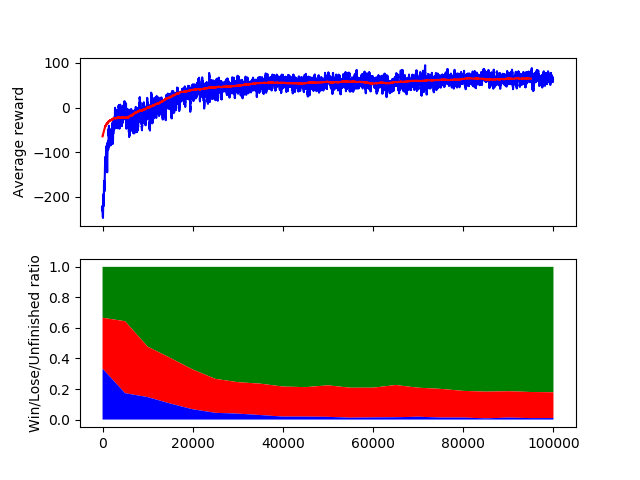
\includegraphics[width=\textwidth]{images/4_4_2_fully.png}
	\caption{Training progress of a $50,50$ fully connected network learning to play on a $4 \times 4$ field with $2$ mines. Win rate is green, red is lose and blue is the unfinished rate averaged over the last $5000$ games. For the average reward blue is averaged over $100$ games and red over $5000$ games.}
	\label{fig:4_4_2_fully}
\end{figure}

Increasing the number of mines also raises the complexity of the game.
Training the agent for $1000000$ games on a $4 \times 4$ field with e.g. $4$ mines results in a win rate of $59.70\%$.
Most of the complexity and thus the decreased win rate lies in the moves needed to win the game.
Winning a game with $4$ mines an average of about $8$ actions are needed.
This is twice the amount 

\begin{figure}
	\centering
	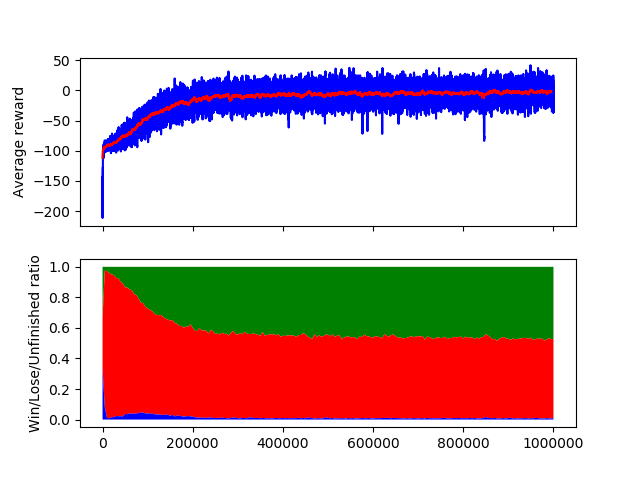
\includegraphics[width=\textwidth]{images/4_4_4_fully.png}
	\caption{Training progress of a $50,50$ fully connected network learning to play on a $4 \times 4$ field with $4$ mines. Win rate is green, red is lose and blue is the unfinished rate averaged over the last $5000$ games. For the average reward blue is averaged over $100$ games and red over $5000$ games.}
	\label{fig:4_4_4_fully}
\end{figure}

As the goal of the project was to play Minesweeper on a `Beginner' level, we increased the size to $5 \times 5$ to see how the pure fully connected network scales with an increased input and action space.
Training the network, progress in Figure~\ref{fig:5_5_5_fully_2million}, needs a lot more games compared to $4 \times 4$.
However after two million games, the agent achieves on $5000$ test games a win rate of $47.78\%$.

\begin{figure}
	\centering
	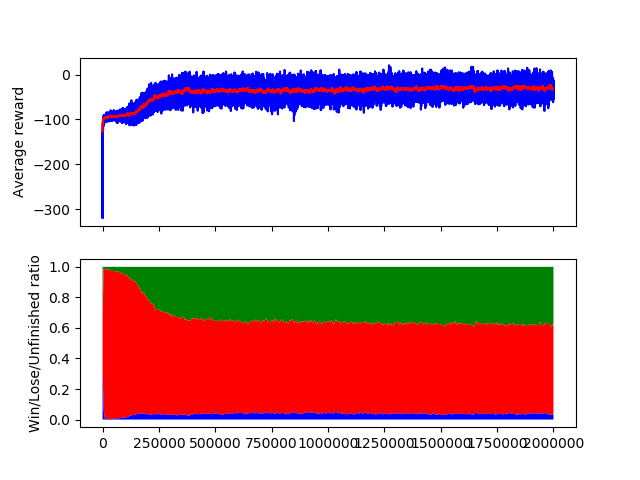
\includegraphics[width=\textwidth]{images/5_5_5_fully_2million.png}
	\caption{Training progress of a $50,50$ fully connected network learning to play on a $5 \times 5$ field with $5$ mines. Win rate is green, red is lose and blue is the unfinished rate averaged over the last $5000$ games. For the average reward blue is averaged over $100$ games and red over $5000$ games.}
	\label{fig:5_5_5_fully_2million}
\end{figure}

As the network topology with $50$ neurons and two layers was just an initial guess, we tried different amounts of neurons and layers to test how it influences the performance.
Two test results are shown in Figure~\ref{fig:layer_test}.
As can be seen, $100$ neurons in one layer are not able to learn Minesweeper as fast as two layers with $50$ neurons each.
Adding a third layer with $50$ neurons increases the complexity of the network resulting in a slower training progress, as can be seen in the bottom of Figure~\ref{fig:layer_test}.
This lead us to choose two fully connected layers for our network.
Doubling the amount of neurons to $100$ on each layer leads to about the same result but increases the computation time.

\begin{figure}
	\centering
	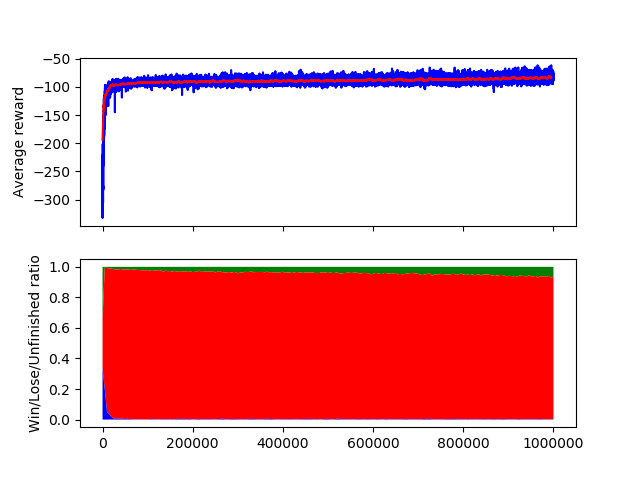
\includegraphics[width=0.8\textwidth]{images/one_layer.png}
	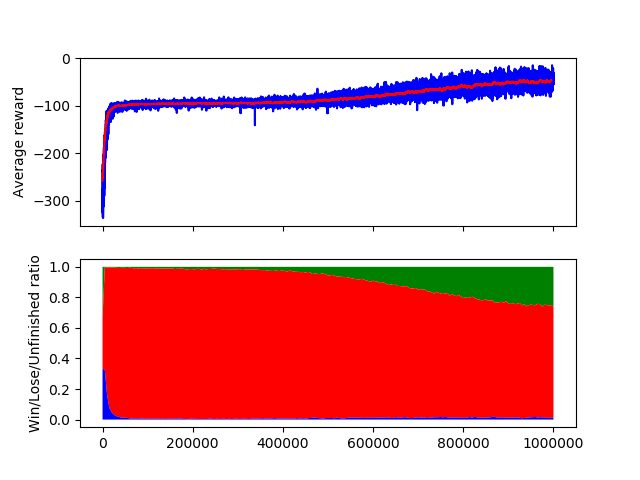
\includegraphics[width=0.8\textwidth]{images/three_layers.png}
	\caption{Training results for one layer network with $100$ neurons (top) and a three layer network with $50$ neurons on each layer. Each network was trained for $1000000$ episodes.}
	\label{fig:layer_test}
\end{figure}

One of the main problems with neural network is the immense amount of parameters needed to be set by the person training the network.
Most of the parameters can not be tested alone but they often interact with other parameters.
This creates dependencies and it is just not possible to evaluate the whole spectrum of possible parameters.


\chapter{Conclusion}

\section{Comparison}

\section{Conclusion}

\section{Future Work}

%%
%% Anhänge
%%
\appendix
\chapter{Quelltexte}

In diesem Anhang sind einige wichtige Quelltexte aufgeführt.

\begin{lstlisting}
public class Hello {
    public static void main(String[] args) {
        System.out.println("Hello World");
    }
}
\end{lstlisting}



%%
%% Nachspann
%%
\backmatter


%%
%% Literaturverzeichnis
%%
\bibliography{bibliography}


%%
%% Versicherung
%%
\cleardoublepage
\thispagestyle{empty}

Name: \fullname \hfill Matrikelnummer: \matnr \vspace{2cm}

\minisec{Erklärung}

Ich erkläre, dass ich die Arbeit selbständig verfasst und keine anderen als die angegebenen Quellen und Hilfsmittel verwendet habe.\vspace{2cm}

Ulm, den \dotfill

\hfill {\footnotesize \fullname}
\end{document}
